% --------------------------------------------------------------
% This is all preamble stuff that you don't have to worry about.
% Head down to where it says "Start here"
% --------------------------------------------------------------
 
\documentclass[12pt]{article}
 
\usepackage[margin=1in]{geometry} 
\usepackage{amsmath,amsthm,amssymb}
\usepackage[margin=1in]{geometry} 
\usepackage{amsmath,amsthm,amssymb}
\usepackage[english]{babel} %Castellanización
\usepackage[T1]{fontenc} %escribe lo del teclado
\usepackage[utf8]{inputenc} %Reconoce algunos símbolos
\usepackage{lmodern} %optimiza algunas fuentes
\usepackage{graphicx}
\graphicspath{ {images/} }
\usepackage{hyperref} % Uso de links
\begin{document}
 
% --------------------------------------------------------------
%                         Start here
% --------------------------------------------------------------
 
\title{COMP9318 (19T1) Assignment 1}
\author{Chris Joy (z5113243)}

\maketitle
\section{Curvas}
A continuación se presenta la representación gráfica de dos curvas, simultáneamente, cuyas ecuaciones están dadas por:


\
\[\left\{ \begin{array}{rcl}
f_{1}=(cos(t),tan(t))
\\
f_{2}=(tan(t),sin(t)) 
& 
\end{array}
\right. \]


% Y este la incluye con etiqueta y pie de imagen
\begin{figure}[h]
\centering
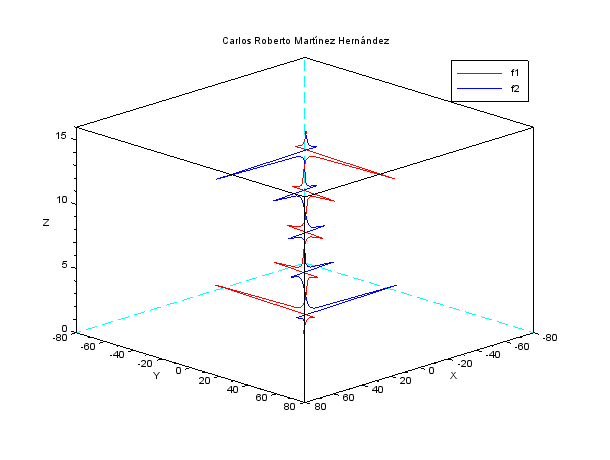
\includegraphics[scale=0.65]{Images/curva4.png} 
\caption{Gráfica de dos funciones simultáneas}
\label{etiqueta}
\end{figure}


% --------------------------------------------------------------
%     You don't have to mess with anything below this line.
% --------------------------------------------------------------
 
\end{document}